\section{Evaluation}
\label{sec:evaluation}

  \subsection{Exhaustive search vs \atl orthogonal search}
  \label{sec:exhaustiveVSorthogonal}
    In this section, we compare the result of \atl orthogonal search with the best of exhaustive
    search. The search time, generated code performance, and selected parameters are listed in Figure
    \ref{fig:exhaustiveVsorthogonal}.\par
    Except for the two ARM processors, it takes around one to three minutes for ATLAS orthogonal search 
    to generate its best code. Considering that we only search for single precision, real number general 
    matrix multiplication, we haven't run double precision, complext number or some other benchmarks 
    like transpose matrix kernel, matrix vector kernel, big matrix kernel, rank-1 matrix kernel etc, installing 
    ATLAS may take hours to finish. The orthogonal search is still too slow to end user.\par
    Column \textit{exhaustive best} and \textit{ATLAS best} list the FMLOPS performance of generated code from
    both search strategy. The ratio of ATLAS over exhaustive is in the last column. On 8 platforms, 
    ATLAS is able to generate code with >90\% of best performance. Three platforms has only around 60\% of 
    best performance. The two parameter columns list the selected paraeters in the order of $(NB, MU, NU, KU)$.\par
    Note for the two MAC platform that, the two middle parameters (MU, NU) are so large that it exceeds 
    the register requirement of \[ MU*NU + MU + NU + LS < NR \]. Thus ATLAS orthogonal search is not able 
    to find it. Currently we do not have a clear explanation to this. One guess is that, the CORE i7 processors
    have more physical registers than ISA architecture register. The ISA is only able to use or identify 32 registers.
    However due to register renaming, it can make use of more than 32 registers and the extra registers are not visible 
    to softwares.\par
     



  \begin{figure*}[tbhp]
    \centering
    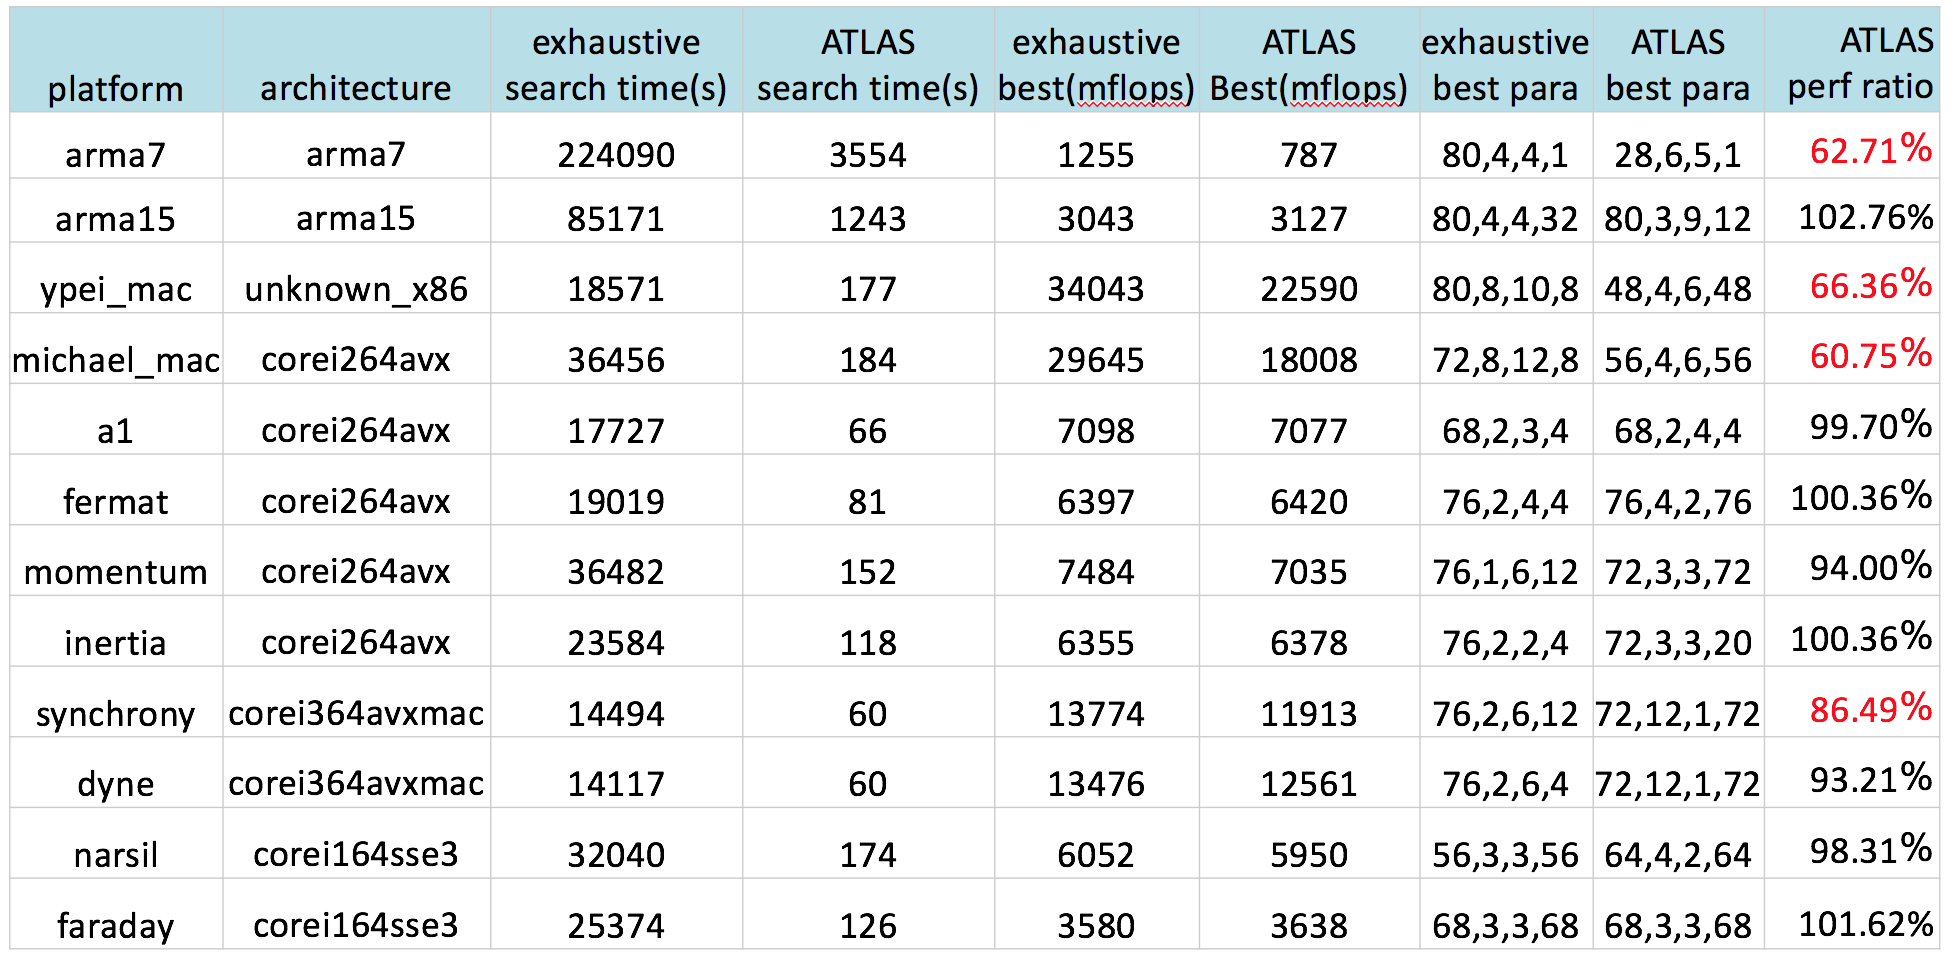
\includegraphics[width=0.9\textwidth]{images/exhaustiveVsorthogonal.png}
    \caption{Searching time comparison between exhaustive search and \atl orthogonal search}
    \label{fig:exhaustiveVsorthogonal}
  \end{figure*}

  \subsection{GEMM performance model}
  \label{sec:GEMMperf}

  \subsection{Capri-based ATLAS searching time}
  \label{sec:capri_atlas_searching}

  \begin{figure*}[tbhp]
    \centering
    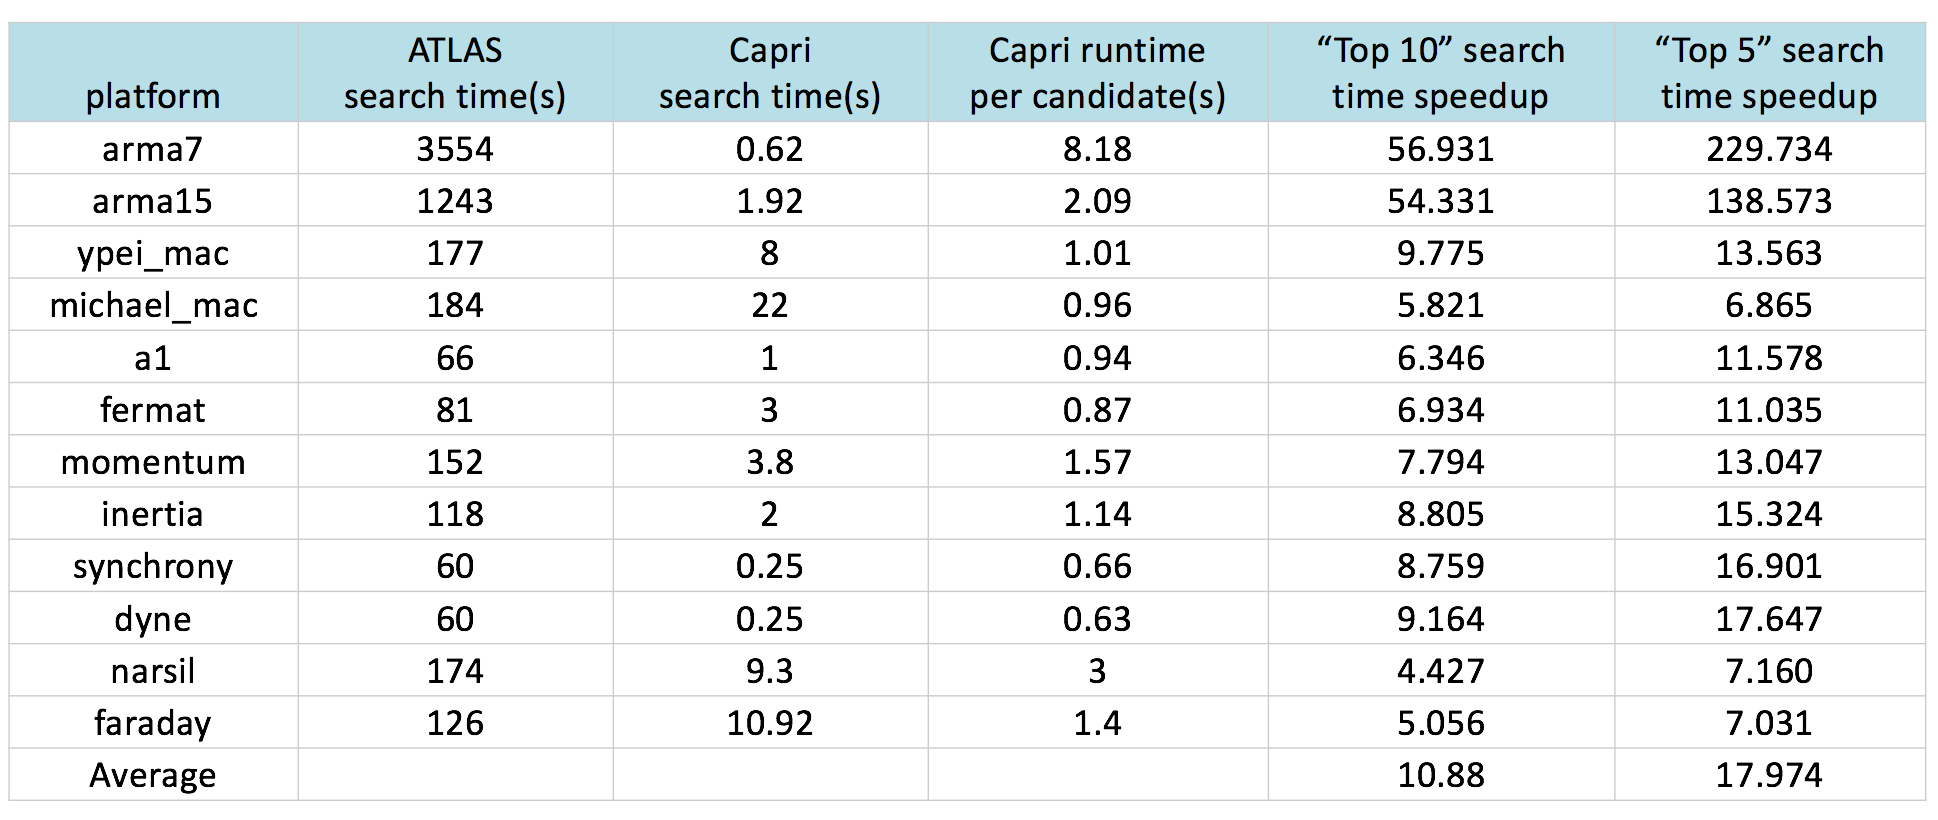
\includegraphics[width=0.9\textwidth]{images/timespeedup.png}
    \caption{Capri-based ATLAS searching time speedup}
    \label{fig:platforms}
  \end{figure*}

  \subsection{Capri-based ATLAS performance}
  \label{sec:capri_atlas_performance}

  \begin{figure*}[tbhp]
    \centering
    \begin{subfigure}[b]{1.0\linewidth}
      \centering
      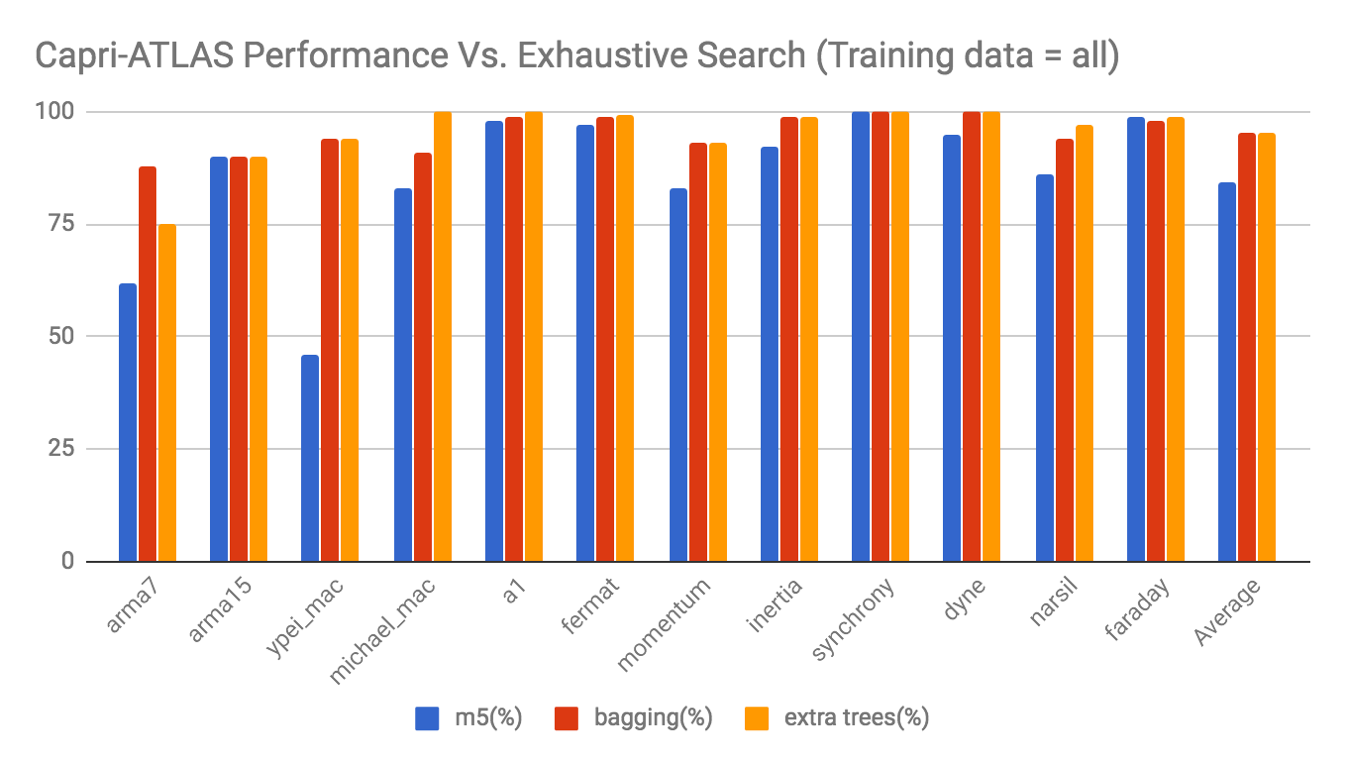
\includegraphics[width=0.9\textwidth]{images/all_perf.png}
      \caption{Training set contains all the platforms except the testing platform}
      \label{fig:all_perf}
    \end{subfigure}
    \begin{subfigure}[b]{1.0\linewidth}
      \centering
      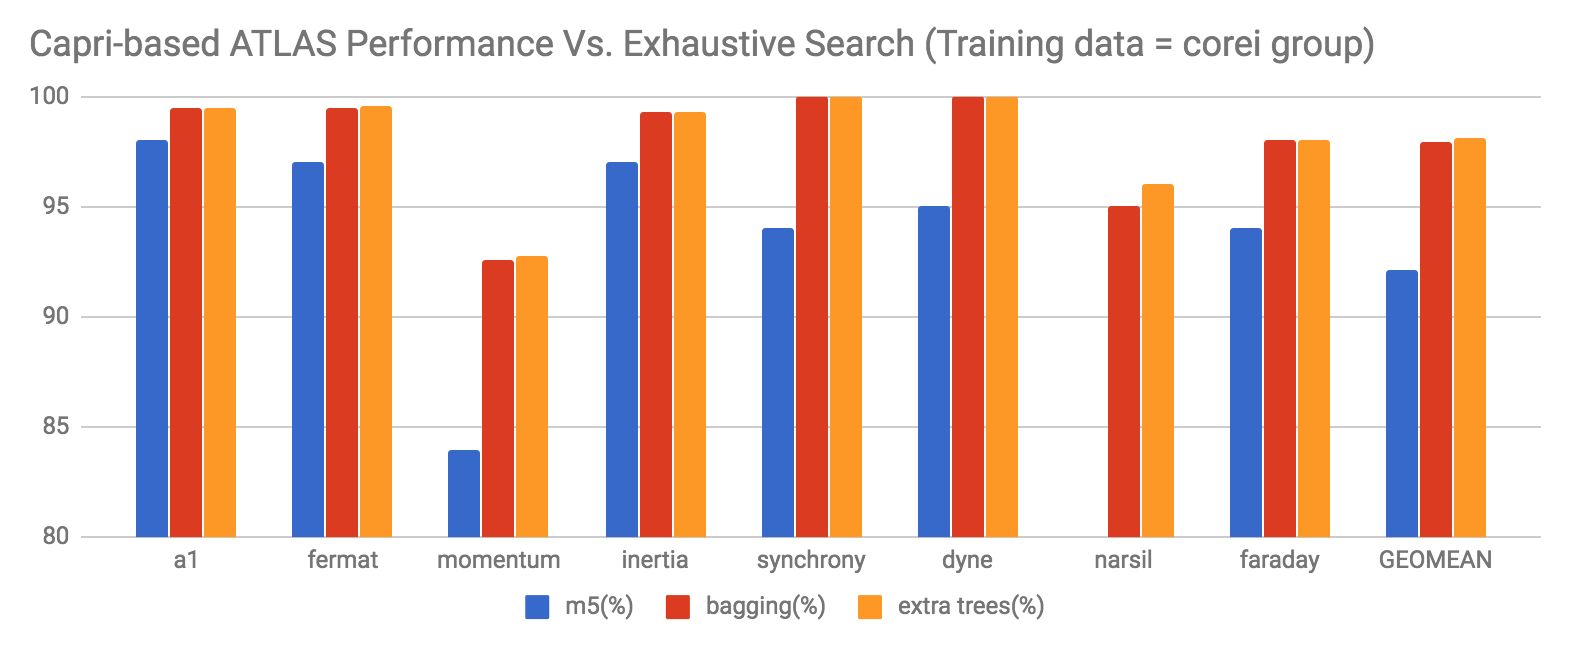
\includegraphics[width=0.9\textwidth]{images/corei_perf.png}
      \caption{Training set contains all the ``corei'' architecture platforms except the testing platform}
      \label{fig:corei_perf}
    \end{subfigure}
    \begin{subfigure}[b]{1.0\linewidth}
      \centering
      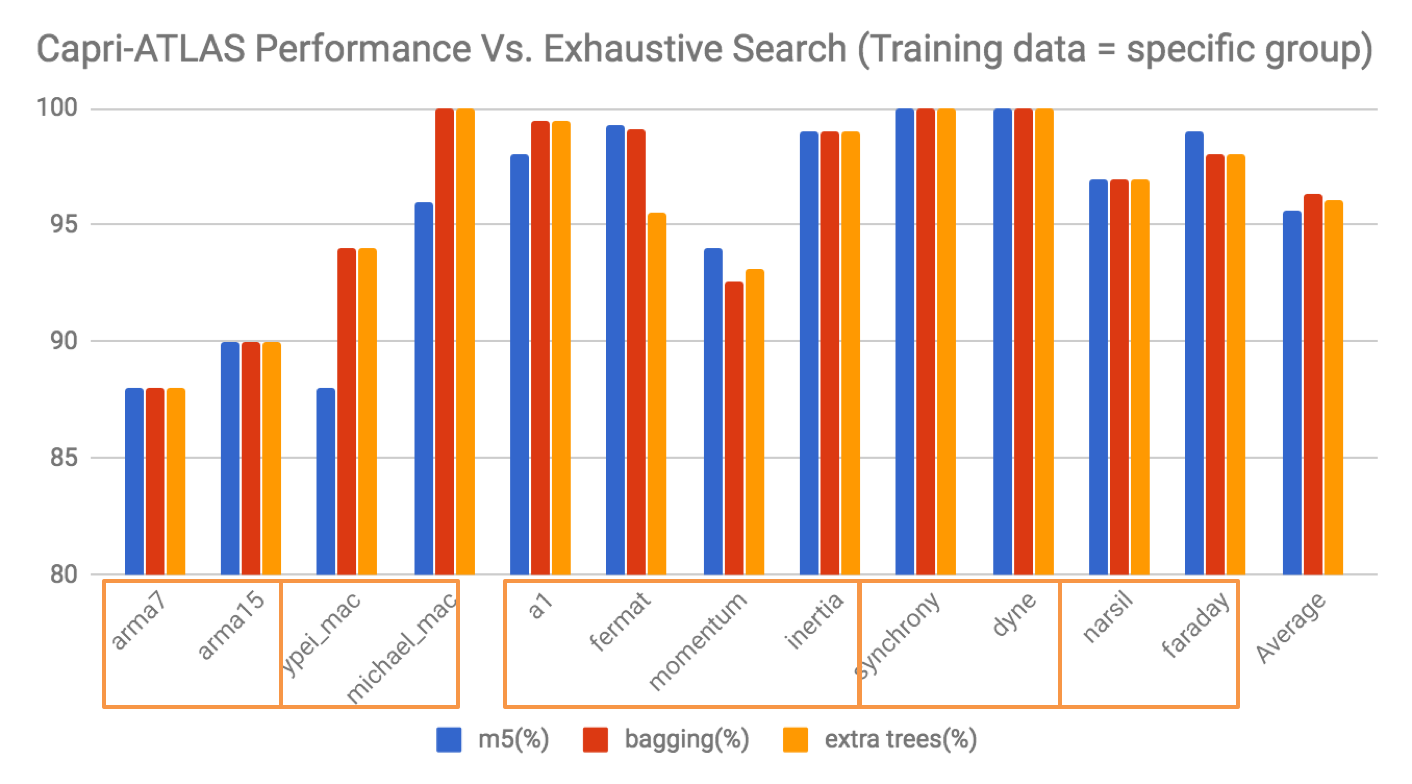
\includegraphics[width=0.9\textwidth]{images/specific_perf.png}
      \caption{Training set contains all the specific platforms except the testing platform}
      \label{fig:specific_perf}
    \end{subfigure}
  \caption{Capri-based \atl design diagram}
  \end{figure*}

  \subsection{Parameter sensitivity}
  \label{sec:parametersensitivity}

    \subsubsection{Training set}
    \label{sec:training_set}

    \subsubsection{Top M constraint}
    \label{sec:top_m}
